\documentclass{beamer}
\usepackage[utf8]{inputenc}

\usetheme{Madrid}
\usecolortheme{default}
\usepackage{amsmath,amssymb,amsfonts,amsthm}
\usepackage{txfonts}
\usepackage{tkz-euclide}
\usepackage{listings}
\usepackage{adjustbox}
\usepackage{array}
\usepackage{tabularx}
\usepackage{gvv}
\usepackage{lmodern}
\usepackage{circuitikz}
\usepackage{tikz}
\usepackage{graphicx}
\usepackage{gensymb} % For using \degree symbol

\setbeamertemplate{page number in head/foot}[totalframenumber]

% Title Information
\title{2.10.32}
\date{September 29, 2025}
\author{ADHARVAN KSHATHRIYA BOMMAGANI - EE25BTECH11003}

\begin{document}

% Title Slide
\frame{\titlepage}

% Question Slide
\begin{frame}{Question}
Let $\vec{p}$ and $\vec{q}$ be the position vectors of $\vec{P}$ and $\vec{Q}$ respectively, with respect to $\vec{O}$ and $|\vec{p}| = p, |\vec{q}| = q$. 

The points $\vec{R}$ and $\vec{S}$ divide $PQ$ internally and externally in the ratio $2:3$ respectively. If $OR$ and $OS$ are perpendicular, then
\begin{enumerate}[]
    \item $9p^2 = 4q^2$
    \item $4p^2 = 9q^2$
    \item $9p = 4q$
    \item $4p = 9q$
\end{enumerate}
\end{frame}

% Step 1: Position vectors
\begin{frame}{Theoretical Solution}
Since $R$ divides $PQ$ internally in the ratio $2:3$,
\begin{align*}
\vec{R} = \frac{3\vec{p} + 2\vec{q}}{5}.
\end{align*}

Since $S$ divides $PQ$ externally in the ratio $2:3$,
\begin{align*}
\vec{S} = 3\vec{p} - 2\vec{q}.
\end{align*}
\end{frame}

% Step 2: Perpendicular condition
\begin{frame}{Theoretical Solution }
Given $OR \perp OS$, we have
\begin{align*}
\vec{R}^T \vec{S} = 0.
\end{align*}

Substitute $\vec{R}$ and $\vec{S}$:
\begin{align*}
\left(\frac{3\vec{p} + 2\vec{q}}{5}\right)^T (3\vec{p} - 2\vec{q}) = 0.
\end{align*}
\end{frame}

% Step 3: Simplification
\begin{frame}{Theoretical Solution}
Multiply through by $5$:
\begin{align*}
(3\vec{p} + 2\vec{q})^T (3\vec{p} - 2\vec{q}) = 0.
\end{align*}

Expanding:
\begin{align*}
9\vec{p}^T\vec{p} - 6\vec{p}^T\vec{q} + 6\vec{q}^T\vec{p} - 4\vec{q}^T\vec{q} = 0.
\end{align*}

\begin{align*}
9\vec{p}^T\vec{p} - 4\vec{q}^T\vec{q} = 0.
\end{align*}
\end{frame}

% Step 4: Final Result
\begin{frame}{Theoretical Solution}
That is,
\begin{align*}
9\|\vec{p}\|^2 - 4\|\vec{q}\|^2 &= 0 
\quad \implies \quad 
9p^2 = 4q^2.
\end{align*}

\textbf{Answer: (a)} $9p^2 = 4q^2$
\end{frame}

% Step 5: Figure
\begin{frame}{Plot}
\centering
\textbf{Vectors OR and OS with $OR \perp OS$}
\begin{figure}[h!]
    \centering
    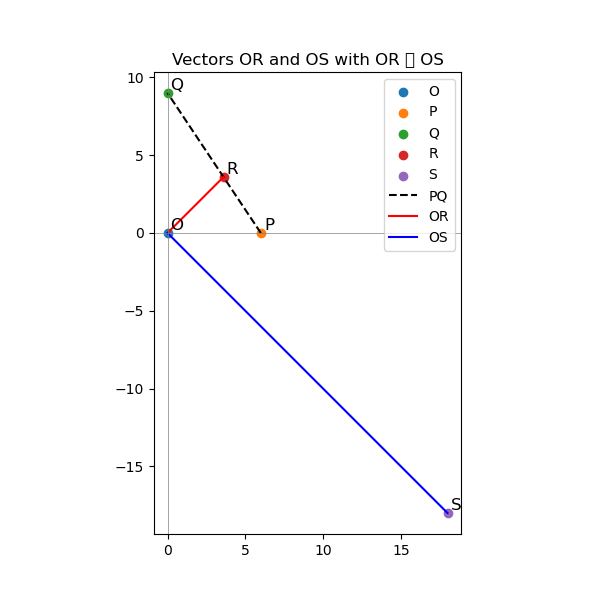
\includegraphics[width=0.6\columnwidth]{figs/fig1.png}
    \caption{Figure for 2.10.32}
\end{figure}
\end{frame}

\end{document}
